% Chapter Template

\chapter{Design} % Main chapter title

\label{Chapter3} % Change X to a consecutive number; for referencing this chapter elsewhere, use \ref{ChapterX}

\lhead{Chapter 3. \emph{Design}} % Change X to a consecutive number; this is for the header on each page - perhaps a shortened title

\section{Modules}
Following modules were identified for development.

\begin{itemize}
	\item Thin client that runs 24x6 and continuously listens and downloads the data from remote server.
	\item Kafka cluster to reliably distribute the data to multiple clients. Each trader gets a unique \emph{group}, which ensures same data is delivered to everyone with equal priority.
	\item A consumer that subscribes to kafka topic and stores the data in persistent storage.
	\item An uploader program that reads that periodically uploads this data to a sql server.
	\item A monitor program that continously checks the health of the thin client and raises alerts
	\item A program called \emph{Enricher} that can be used to read the raw data and republish it with any required changes.
\end{itemize}

\subsection{Thin client}
This client listens to Refinitiv's TIBCO-EMS queue, and immediately publishes the same data to a pre-defined kafka topic. Since Refinitiv expects the queue to be continuously emptied, it is important that the client remains highly available. To maintain low latency, C++ was used

\subsection{Kafka topics}
A pre-defined kafka topic is used to consume the raw data.

Another topic is used by the uploader.

Another topic is used by the enricher.

\subsection{Enricher}
This is used to read the raw data and convert to some other format, such as protobuf etc.

\subsection{SQL}
SQL database was used to maintain historical consistency. The database was partitioned based on quarters, as we found that most queries were made only for previous 30 days.

\section{HLD}
A high level architecture diagram of the proposition is shown in Figure \ref{fig:Architecture Diagram}

\begin{figure}[htbp]
	\centering
	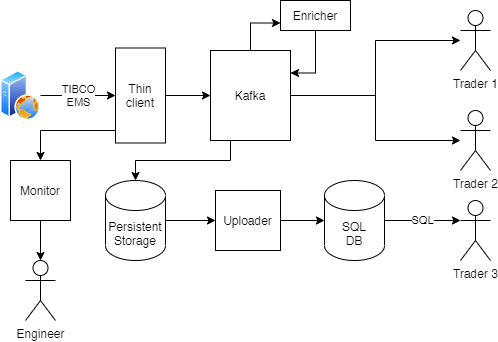
\includegraphics[width=1.0\columnwidth]{Figures/ArchitectureDiagram.png}
	\rule{35em}{0.5pt}
	\caption[Architecture Diagram]{Architecture Diagram of proposed system}
	\label{fig:Architecture Diagram}
\end{figure}
%----------------------------------------------------------------------------------------
%	SECTION 1
%----------------------------------------------------------------------------------------
